\documentclass[sigplan,screen,nonacm]{acmart}
\usepackage{rotating}
\usepackage{tabularray}
\usepackage{color}
\setlength {\marginparwidth }{2cm}
\usepackage[colorinlistoftodos]{todonotes}
\usepackage[
    type={CC},
    modifier={by-nc-sa},
    version={4.0},
]{doclicense}

%% \BibTeX command to typeset BibTeX logo in the docs
\AtBeginDocument{%
  \providecommand\BibTeX{{%
    \normalfont B\kern-0.5em{\scshape i\kern-0.25em b}\kern-0.8em\TeX}}}

%% end of the preamble, start of the body of the document source.

\begin{document}

%%
%% The "title" command has an optional parameter,
%% allowing the author to define a "short title" to be used in page headers.
\title{Using Internet of Things for Wildlife Tracking}

%% "authornote" and "authornotemark" commands
%% used to denote shared contribution to the research.
\author{Collin R. Beane}
\email{beane039@morris.umn.edu}
\affiliation{%
  \institution{Division of Science and Mathematics
    \\
    University of Minnesota, Morris
  }
  \city{Morris}
  \state{Minnesota}
  \country{USA}
  \postcode{56267}
}

%%
%% The abstract is a short summary of the work to be presented in the
%% article.
\begin{abstract}
  This paper provides a comprehensive examination of the utilization of
  Internet of Things (IoT) devices in wildlife management and tracking,
  their evolutionary trajectory, and practical implementation in data
  acquisition. Central to the discussion are key components of IoT networks,
  including Sigfox, Wi-Fi-enabled devices, and IoT-based wireless sensor
  networks, each analyzed for their role and efficacy. Communication
  modalities within IoT frameworks, coupled with an evaluation of protocol
  performance are evaluated.

  Furthermore, this seminar also addresses challenges inherent in wildlife
  data collection methodologies, such as memory constraints, battery life,
  transmission range and rate, and security vulnerabilities within IoT
  ecosystems. By delving into potential solutions and technological
  advancements, this paper aims to contribute to the refinement of wildlife
  monitoring practices, fostering a more robust and effective approach to
  conservation efforts.
  \todo[inline, color=orange]{This is a preliminary abstract, I mainly added it just so I had something.}
\end{abstract}

\doclicenseThis

\keywords{IoT, networking, Wi-Fi, data transmission, data collection,
  animal trackers, Sigfox, WildFi, Biologging, ecology}


%%
%% This command processes the author and affiliation and title
%% information and builds the first part of the formatted document.
\maketitle

\section{Introduction}
\label{sec:introduction}

\section{Background}
\label{sec:Background}

Comprehending the foundational technology behind the Internet of Things (IoT)
is paramount in grasping its applications in wildlife tracking. This section
aims to furnish a concise overview of biologging, the IoT, and their
intersection in wildlife tracking. Additionally, it will explore current and past
technologies employed in biologging, shedding light on their operational
mechanisms and comparative advantages. By delving into the workings of
traditional wildlife tracking technologies, we can evaluate their merits and
demerits, thereby establishing a framework for evaluating the suitability of
IoT solutions for wildlife tracking.

\subsection{What is Biologging?}
\label{subsec:What is Biologging}

Biologging is a concept that gained popularity in the early 2000's and has continued
to play a pivotal role in understanding animal behavior and ecology. Biologging can be
defined as "The investigation of phenomena in or around free-ranging organisms that are beyond
the boundary of our visibility or experience. \cite{boyd2004bio}"
It is a method of tracking animals in the wild using electronic devices that are
attached to the animal. These devices can be used to track the animal's
movements, monitor its behavior, and collect data on its environment. Biologging
emerged as a powerful tool in ecology in a similar way genomics did for the study
of cell and organ function. The obvious difference being that biologging provides
insights into the behavior and functions of various organisms in environments that
can be hostile or difficult to reach for the observer, rather than the function of cells and
organs \cite{boyd2004bio}. The ability to track animals in their natural environment has
provided researchers with a wealth of data that was previously unattainable. This data
has been used to study animal behavior, migration patterns, and the effects of climate change
on various species\cite{10.3389/fevo.2018.00092}. The data collected from biologging
devices has also been used to inform conservation efforts and to help protect endangered
species \cite{cooke2008biotelemetry}. It is important to understand that biologging is
simply the collection of data from animals in the wild, and it is then up to scientists
or conservationists to use the data to answer questions about the animals or to inform
conservation efforts.

\subsection{What are the Other Biologging Methods?}
\label{subsec:What are the Other Biologging Methods?}

Various stratagies have been used in the past to track animals in the wild. Many
implement variations of the same technology within the tracking sensors;
GPS, accelerometers, and magnetometers are the most common sensors used in
biologging devices. These data from these sensors help researchers understand
the animal's  speed, direction, and position, which allows for a 3D mapping of
positions\cite{Kidangoor_2024}. The compilation of this data can be seen in Figure ~\ref{fig:prairie_dog_3D_movement}
from the Smithsonian's National Zoo and Conservation Biology Institute, which
shows the 3D movement of a prairie dogs.
\begin{figure}[htbp]
  \centering
  \fbox{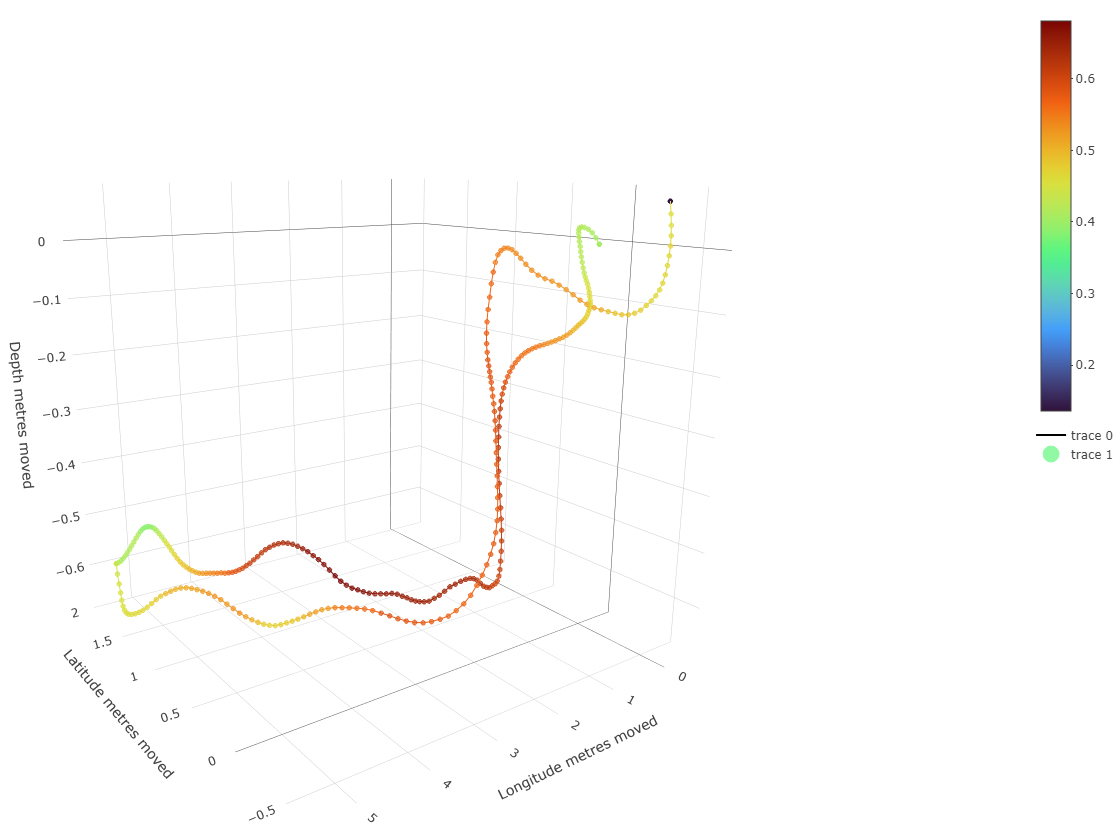
\includegraphics[width=.9\columnwidth]{prairie_dog_map.jpg}}
  \caption{3D movement of a prairie dog \cite{Kidangoor_2024}}
  \label{fig:prairie_dog_3D_movement}
\end{figure}
Most biologging trackers will implement these types of sensors, but the
implementation of these sensors can vary greatly. More importantly, the
communication of the data from these sensors can vary greatly. One of the
most popular methods for transmitting data is the use of cellular networks.
A study conducted by a professor from UC Irvine tested the use of cellular
networks to analyze the pollution levels in the San Jose area by using pigeons
equipped with GPS and automotive emissions sensors \cite{Martin_2006}. Professor
Da Costa had to pay about 10 cents for each message transmitted, and two
messages are sent every minute by each pigeon\cite{Martin_2006}. This leads into one of the biggest
disadvantages of using cellular networks: cost. Another obvious disadvantage
is that cellular networks are not available in all areas, and the range of
cellular networks is limited. It is also practically impossible for researchers
to improve the range of cellular networks by adding more cell towers to cover
their study area. Radio frequency is another technology that has been used to
transmit data from biologging devices for decades. The use of radio frequency
to transmit data from biologging devices requires a receiver to be within range
of the transmitter, and the range of the transmitter is limited by the power of
the transmitter and the frequency of the radio waves. The receiver and transmitter
used by Cooke et al. on marine animals had an effective range of 5 to 1000m and 
is only able to transmit periodic tracking records or time stamped data from loggers
\cite{cooke2012biotelemetry}. This falls short of the capabilities of IoT enabled 
biologging devices using LPWAN networks, which are able to transmit data in real time, and can transmit 
data over much longer distances. 

\subsection{What is WLAN?}
\label{subsec:What is WLAN?}

Understanding the basics of how a wireless networks transmits data is important to understanding 
the reasoning behind using it for biologging. Wireless networks, like WLAN (WiFi), 
works by encoding data into a binary form so it can be sent across a radio frequency to another 
wireless enabled device. Ones and zeroes are represented by different amplitudes of radio waves 
and are received by another device\cite{Ghimire_2023}. There are many frequencies that can 
be used as a medium to send this data, the most popular being 2.4GHz and 5GHz. However, 6GHz 
frequencies are becoming more popular for it's ability to transmit data at faster rates. In general, 
as frequency increases, range is sacrificed for higher data rates\cite{Netgear}. Data rates are 
higher because the radio waves are being received in higher 
frequency, meaning more ones and zeroes are being received every second. In 
some cases, speed is not everything, and range is more important, in this case, a lower frequency 
is a better choice. Sub gigahertz(GHz) frequencies are used in LPWAN networks for this reason. They 
are able to achieve ranges upwards of 40km at the cost of data rates, LPWAN networks are explored futher 
in section ~\ref{subsec:Low Power Wide Area Networks (LPWAN)}

\subsection{What is the Internet of Things?}
\label{subsec:What is the Internet of Things}

The Internet of Things (IoT) represents a transformative shift in the
realm of technology, encompassing a vast array of physical objects empowered
with sensors and software to interact autonomously. These objects collect and
exchange data through network connectivity. In essence, IoT devices, ranging
from commonplace gadgets to sophisticated systems, have the capability to
interface with the internet or communicate wirelessly, thereby facilitating
seamless integration into various facets of daily life. The IoT has been
applied to a wide range of fields, including healthcare, agriculture,
manufacturing, and most important to this paper, wildlife monitoring.
The fundamental structure of an IoT system is comprised of three
interconnected layers: the perception layer, the network layer, and the
application layer\cite{kumar2019internet}. The perception layer is responsible for collecting data
from the environment, which is then transmitted to the application layer via the network layer.
The transmission layer can use a variety of different methods to transmit data, the two most common being
ethernet/WiFi, and cellular networks like 5G and LTE\cite{greengard2021internet}. Lastly, the application
layer is responsible for doing something with the data, such as graph positional data from an
animals GPS sensor. The physical implementation of these layers
can vary greatly, but in general, the perception layer consists of a sensor or device that can
output a signal to be received by a gateway device(the most common gateway device for
the average person would be a wireless router). The gateway device is connected to
the internet using one of the aforementioned methods, and it is responsible for
receiving the data from the perception layer device and transmitting it to the application
layer, which could be a database to store the data, or a web application to display
the data\cite{kumar2019internet}. These three theoretical layers are important in understanding the IoT,
and how it can be used in wildlife tracking. The Wild-Fi biologging tag, is a prime example 
of how these three layers are implemented in a biologging device and is visually explained 
by figure ~\ref{fig:wild-fi_IoT_diagram}.

\section{Components of a IoT Biologging System}
\label{sec:Components of a IoT Biologging Device}

\subsection{The Sensor Device}
\label{subsec:The Sensor Device}


\section{Networking}
\label{sec:Networking}

The networking of a IoT based biologging system is crucial in ensuring safe and
efficient data transmission. The networks used in a biologging system
are responsible for transmitting data from the sensor device to the application
layer, and are also responsible for ensuring that the data is transmitted
safely and securely. The two most popular types of networking protocols used in
biologging systems are Low Power Wide Area Networks (LPWAN) and Traditional Wifi.
These two types of networks have their own advantages and disadvantages, and
the choice of which network to use is dependent on the specific use case. No
matter what method is used, the networking must be able to transmit data over 
long distances, and they must be able to do so in a secure way. The security 
of the data is especially important in a biologging system, as the data being 
transmitted is often sensitive and can be used to track the location of an animal, 
which in the hand of an illegal hunter, could be disastrous.

\subsection{Low Power Wide Area Networks (LPWAN)}
\label{subsec:Low Power Wide Area Networks (LPWAN)}

LPWAN networks provide a few benefits compared to a traditional mesh wifi network, 
the primary benefit being that LPWAN networks are able to transmit data over much 
longer distances than a traditional mesh wifi network. This is especially important 
in a biologging system, as the animals being tracked are often in vast, remote areas 
where a 200m range would not be sufficient. LPWAN networks typically utilize sub 
GHz frequencies and ultra-narrow band modulation to transmit data over long distances
\cite{yousuf2018throughput}. Proprietary LPWAN networks like the SigFox network are 
popular and designed to handle up to a million IoT devices using only a single gateway. 
These services are subscription based, and the cost of the service is based on the 
number of devices that are used in the network. On the other hand, there are LPWAN 
standards that exist to allow in house development of an LPWAN network. The 
LoRaWAN protocol is one of the most popular LPWAN standards, and it is used by 
many to implement their own LPWAN networks\cite{LoRa_Alliance®_2023}. Both of these 
network solutions are explored further in subsections \ref{subsec:SigFox} and 
\ref{subsec:LoRaWAN}.

\subsubsection{SigFox}
\label{subsec:SigFox}

The SigFox network is a proprietary LPWAN 
network that is used for IoT systems, and it can be used to cover an area as 
big as Belgium ($30,600 km^2$) with only seven base stations \cite{wild2023multi}. 
The node device in a SigFox network is able to transmit 6 messages per hour, 
each having a maximum size of 12 bytes. While 12 bytes may seem limiting, it is 
sufficient for transmitting the GPS coordinates of an animal, as well as other 
sensor data such as temperature\cite{wild2023multi}. The SigFox company also offers 
the Atlas technology which uses the signal strength and location of the receiving 
base station to calculate an approximate location of the node device, which frees up 
the node device from having to explicitly send GPS data, allowing for other sensor data 
to be sent instead\cite{wild2023multi}. 
\begin{figure}[htbp]
  \centering
  \fbox{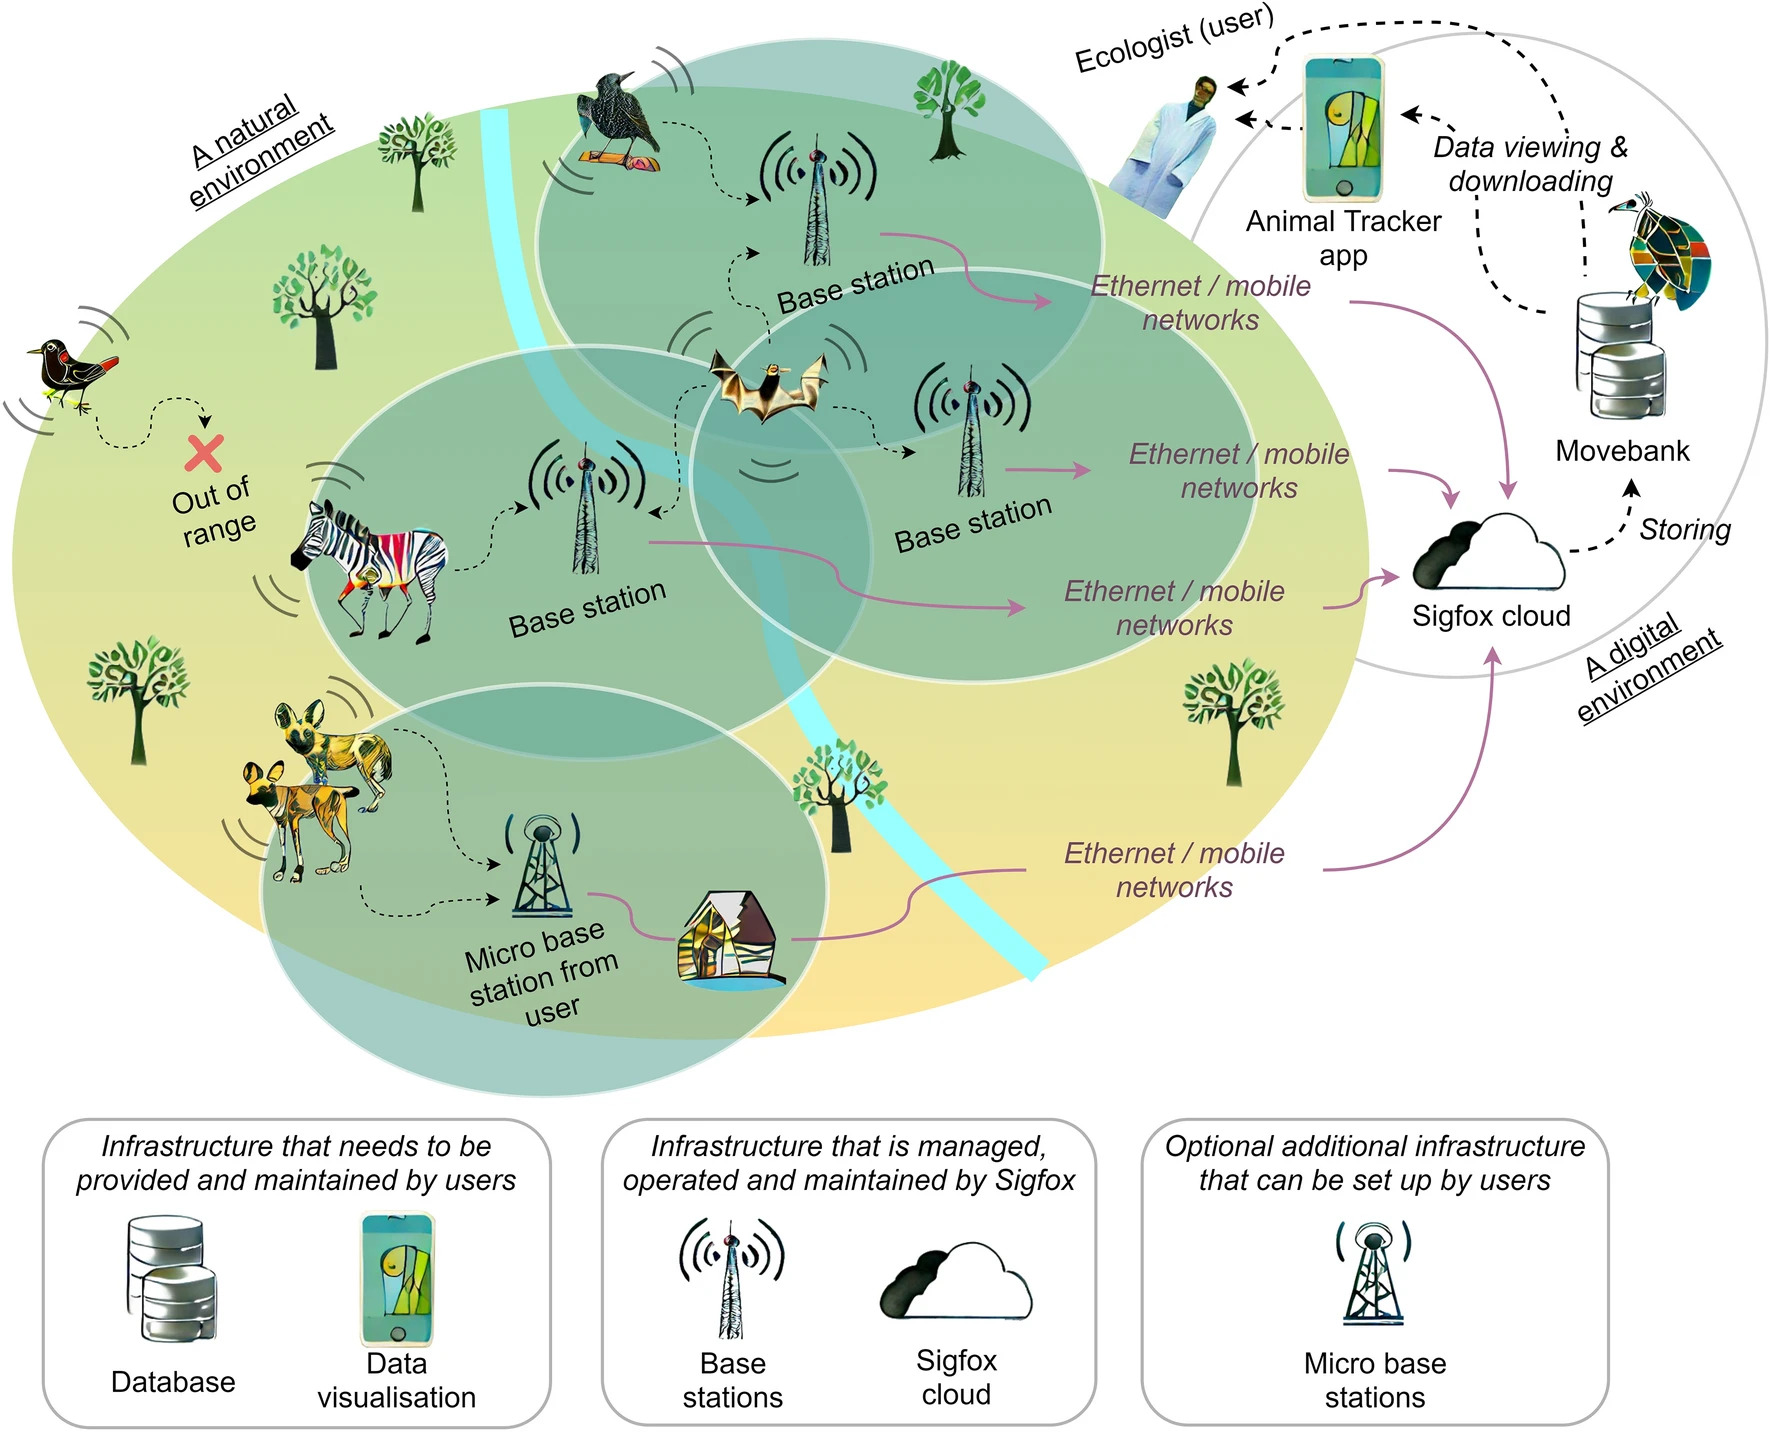
\includegraphics[width=.9\columnwidth]{SigfoxNetworkMap.jpg}}
  \caption{SigFox network infrastructure\cite{wild2023multi}}
  \label{fig:SigFox_infrastructure}
\end{figure}
Ultra-Narrow bands (UNB) are used in the SigFox 
network and many other LPWAN networks, which allows for the transmission of data
over long distances, and the use of UNB also allows for the use of low power
transmitters, which is important in a biologging system, as the devices are
often attached to animals and must be as small and light as possible.
UNB works by using a low radio frequency(868.034MHz to 868.226MHz), and transmits data three 
times on different channels at different times, which ensures a message is received 
and robustness to interferences\cite{LavricSigfoxCommunication}. One of the greatest 
benefits of UNB is that it allows for the use of low power transmitters, which are able 
to have incredibly long battery lives. Using the specifications of SigFox's UNB 
network, a node is able to send 140 packets per day, and the power consumption is 
between 19 and 49 mA, two AAA batteries are able to power a node up to 6.5 years
\cite{LavricSigfoxCommunication}. Because SigFox is a proprietary network, end users 
do not maintain the base stations or connection to the SigFox cloud: they only need to 
design their devices within the SigFox specifications and connect them to the SigFox network. 
An overview of the SigFox infrastructure and how it can be applied to biologging 
is shown in Figure ~\ref{fig:SigFox_infrastructure}.

\subsubsection{LoRa}
\label{subsec:LoRa}

The LoRa and SigFox networks have many similarities in how they are structured 
and operated, however there are some key differences. The transmission modulation 
technique used by LoRa is called CHIRP(Compressed High Intensity Radar Pulse) spread 
spectrum, and it is different from the frequency hopping technique that the SigFox 
network uses. Where frequency hopping transmits signals at a constant frequency before 
hopping to a different frequency, chirp modulates by increasing or decreasing it's 
frequency over time, this can be done both linearly or not\cite{ghoslya2017lora}. The 
spreading factor determines how quickly this modulation takes place; LoRa uses spreading 
factors SF7 to SF12, the larger the spreading factor, the slower the modulation.
How these spreading factors compare to each other is shown in Figure ~\ref{fig:Chirp}. 
The main tradeoffs between spreading factors is the range and data rate of the network, as the 
spreading factor increases, the range of the network increases, but the data rate decreases\cite{erturk2019survey}. 
The spreading factor then becomes a critical factor in the design of a LoRa network, as 
the spreading factor is directly related to the range and data rate of the network, so it should 
be chosen wisely to fit the needs of the specific use case. Because the frequency is constantly 
changing, chirp is able to tolerate interference better than that of the frequency hopping 
technique that the SigFox network uses.

\begin{figure}[htbp]
  \centering
  \fbox{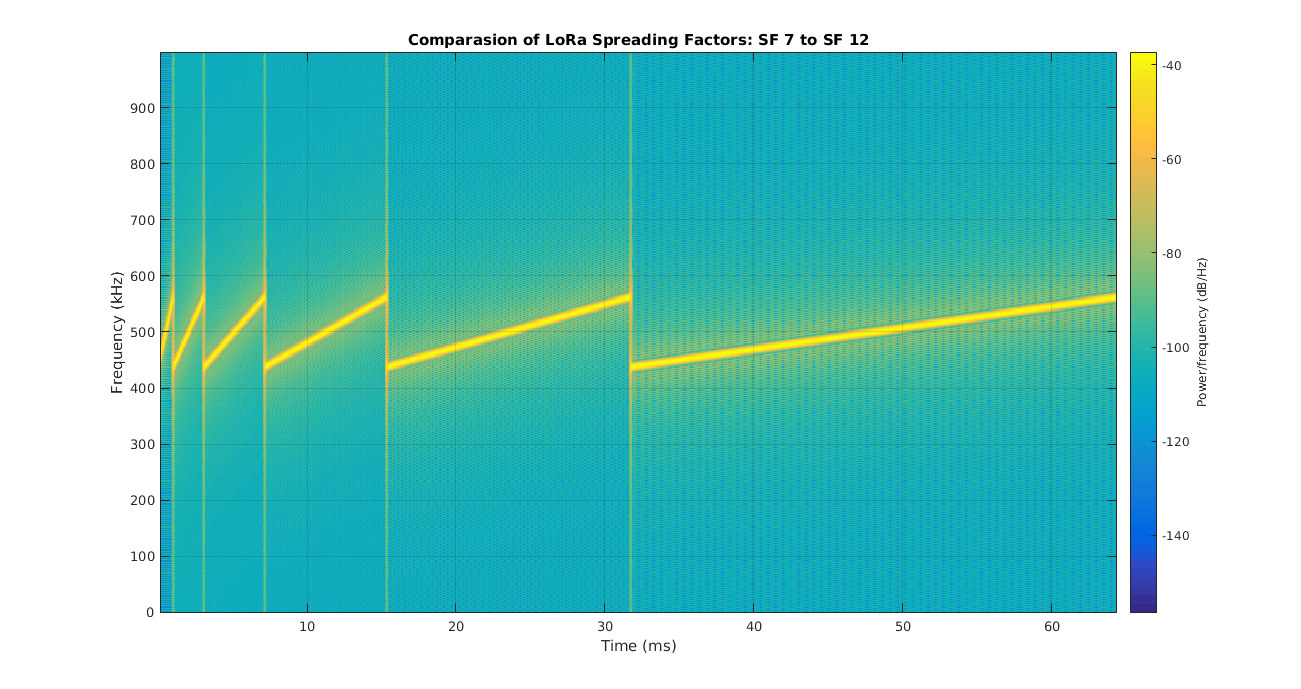
\includegraphics[width=.9\columnwidth]{Chirp.png}}
  \caption{Chirp Spread Spectrum Spreading factors\cite{ghoslya2017lora}}
  \label{fig:Chirp}
\end{figure}

\subsection{Traditional Wifi (WLAN)}
\label{subsec:Traditional Wifi (WLAN)}

A more traditional Wifi network is another method that is used by some companies to 
implement biologging systems. There are some useful benefits to using a traditional 
Wifi network over an alternative like LoRa or LPWAN; The biggest of which is data 
transfer rate. However, because traditional Wifi uses 2.4/5/6 GHz frequencies, the range is much more limited 
than that of a LPWAN network, and the power consumption is higher. The WildFi biologging system designed by 
Timm Wild and his colleagues is just one example of a device that uses traditional 
WLAN to collect data from a biologging device. Wild is also the leading member of the 
team that studied the use of the SigFox network for a IoT based biologging system, and 
claimed that the data transmission capacity was one of the reasons that they chose to 
investigate the use of a traditional Wifi network for biologging\cite{wild2023internet}. 
The WildFi tags and others like it, connect and communicate by using a traditional wireless 
local area network (WLAN), which provides a versatile way for tags to offload collected data. 
As seen in Figure ~\ref{fig:wild-fi_IoT_diagram}, the WildFi tag has the capability to 
connect to a WLAN router, smartphone hotspot, specially designed gateway, and more.
\begin{figure}[htbp]
  \centering
  \fbox{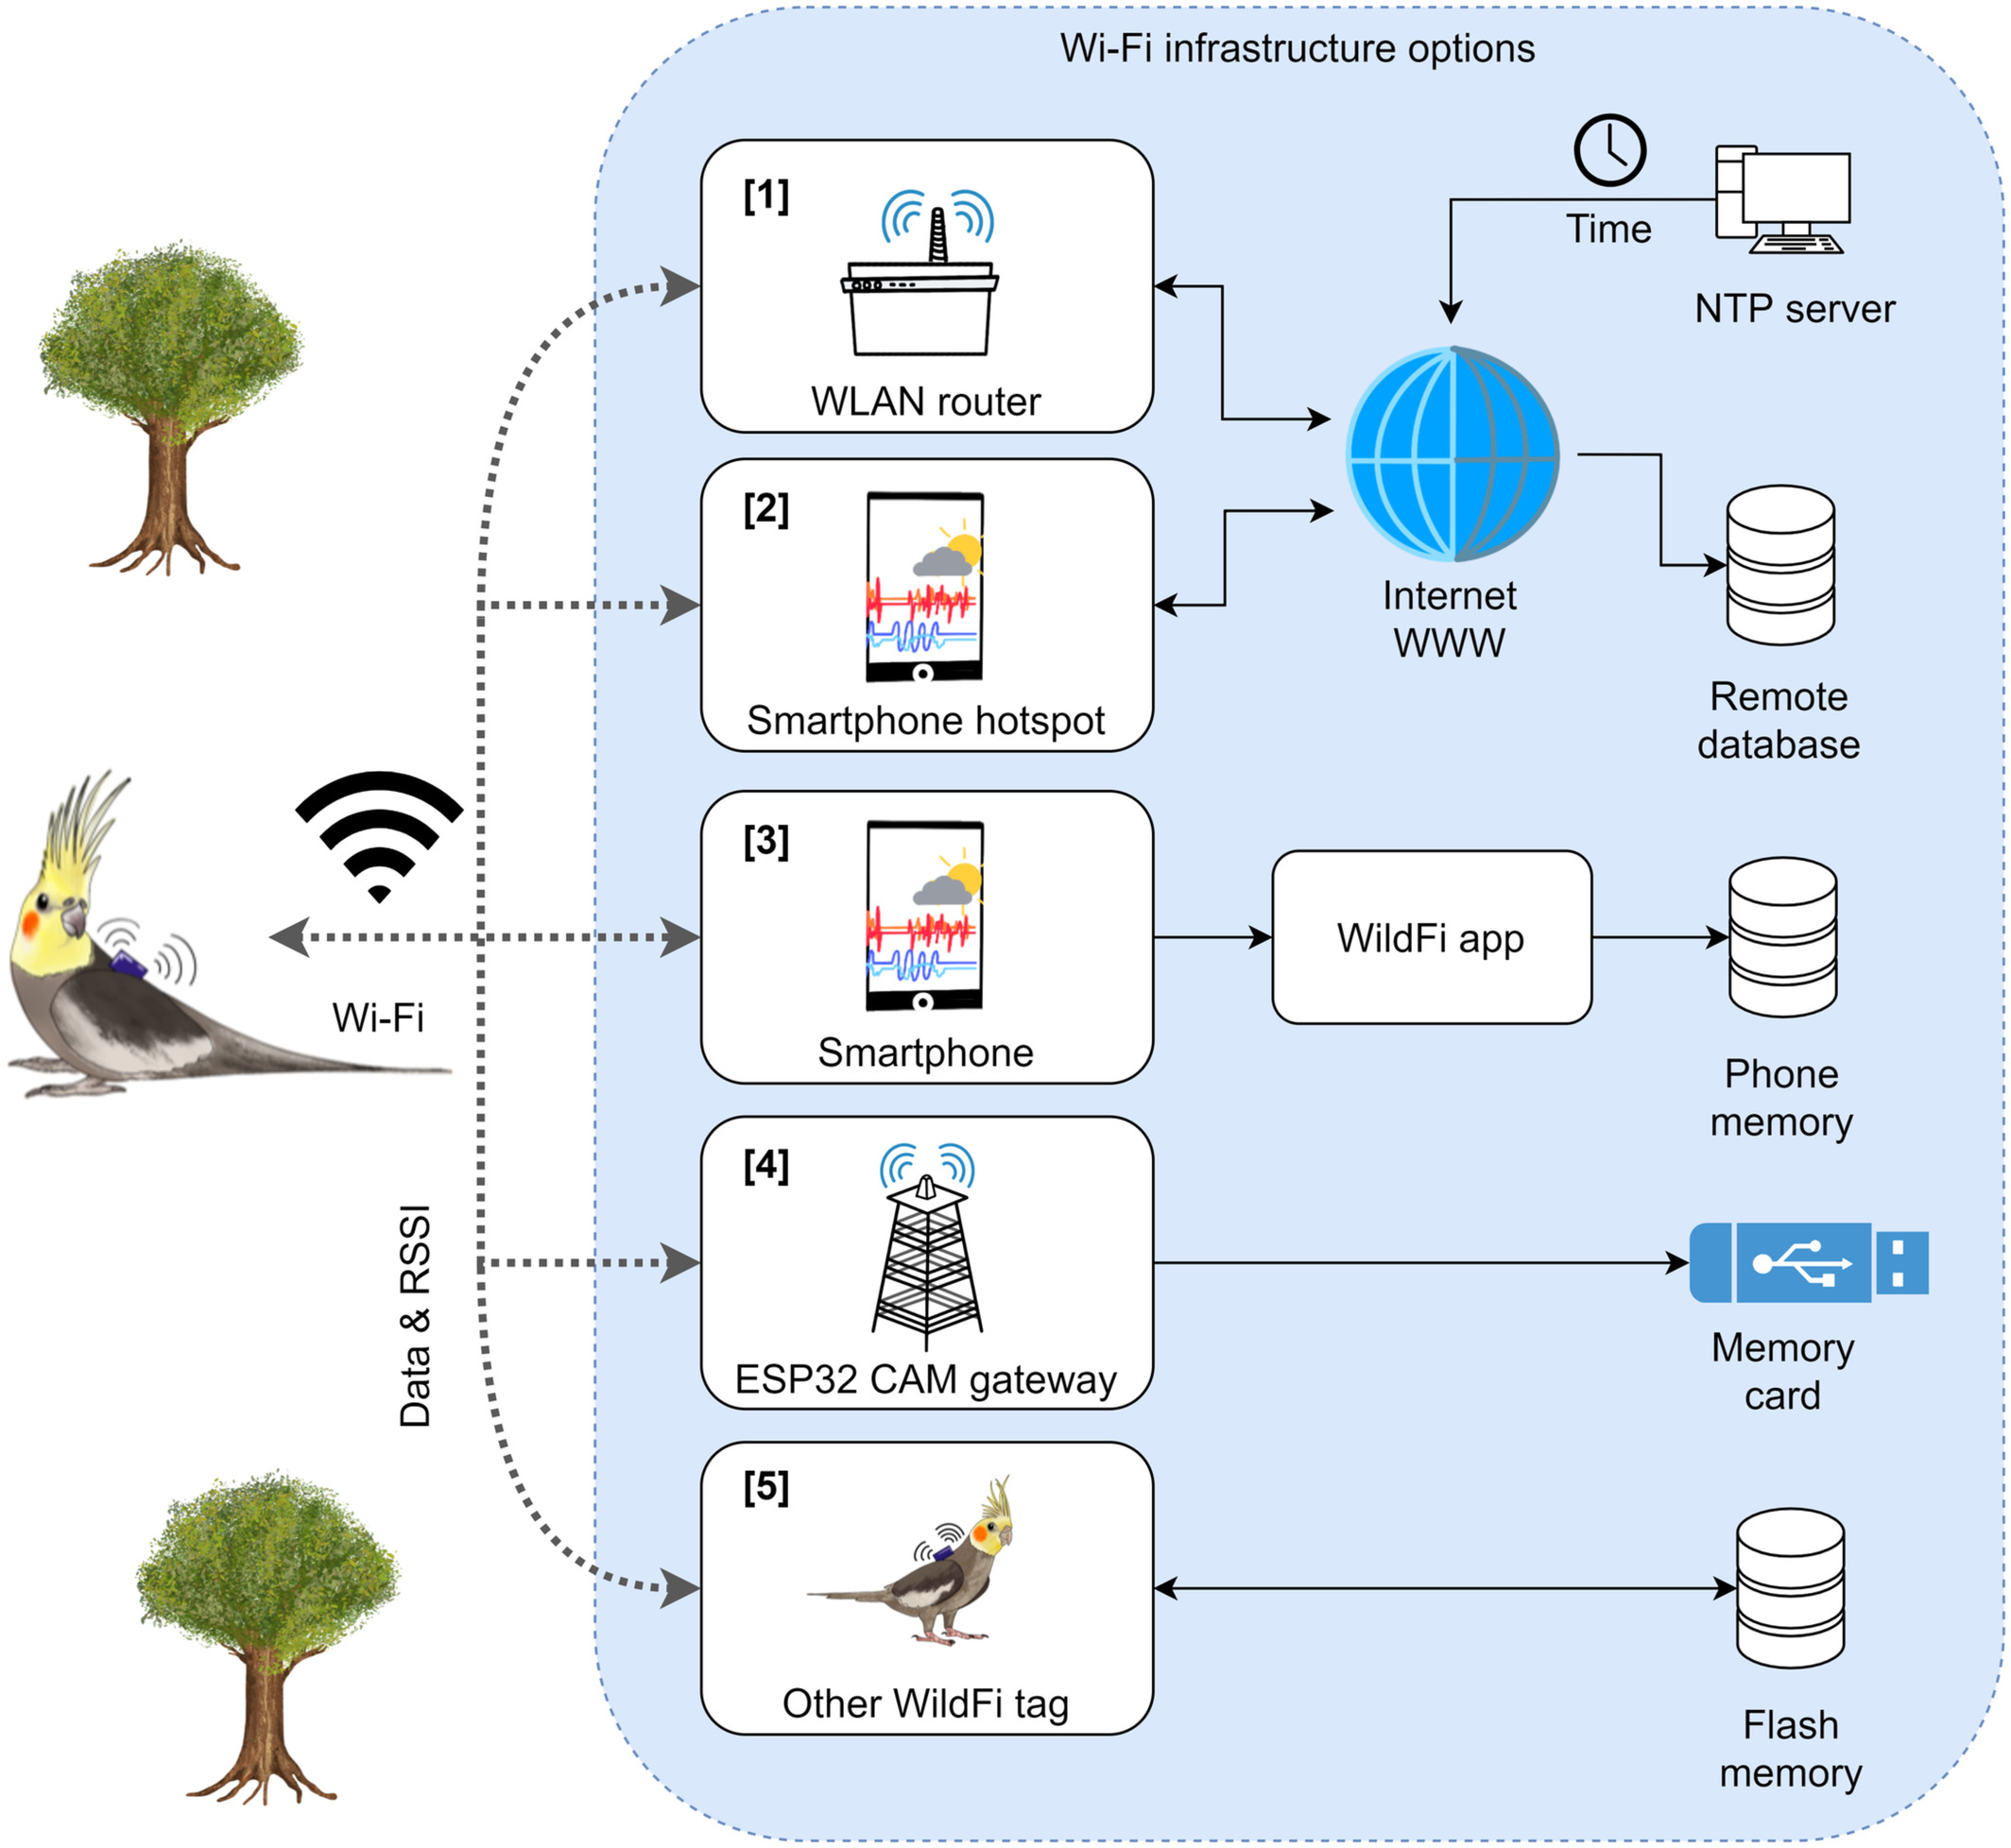
\includegraphics[width=.9\columnwidth]{WildFi_IoT.jpg}}
  \caption{Wild-fi IoT infrastructure overview \cite{wild2023internet}}
  \label{fig:wild-fi_IoT_diagram}
\end{figure}
When the tags establish a connection to one of these devices, data is packaged, encrypted, 
and transmitted to the receiving device. From there, the data can either be stored on device 
to be physically collected, or uploaded to a remote database. When connected to a ESP32 CAM 
gateway and the data is stored locally, a transmission rate of 230 kByte/s can be achieved at 
a distance up to 200m and only consume 108mA using a WildFi tag\cite{wild2023internet}. This 
is more power consumption than a LPWAN based device, however the energy cost per byte 
transmitted is lower than a LPWAN based device. Wild et. al claim that using a traditional 
Wifi network with a logging device that has a 70mAh battery and a small solar panel, data can 
be transmitted 24 hours a day for an entire lifetime of an animal\cite{wild2023internet}.

\subsection{Security}
\label{subsec:Security}

The security of these networks is a critical factor in the design of a biologging system, as 
the data being transmitted is often sensitive and can be used to track the location of an animal, 
which in the hand of an illegal hunter, could be disastrous. While much of the security of the 
data is in the design of the physical device and it's software, the networks being used also need to 
be secure and safe. The security of the physical device is important in the event that a node 
device is lost or stolen.

\subsubsection{SigFox and LoRa Security}
\label{subsec:SigFox and LoRa Security}

Both the SigFox and LoRa network ensure safe data transmission by using AES (Advanced Encryption Standard) 
128 for end-to-end encryption. With this encryption method, a 128 bit key is used to encrypt the data from 
node device and a key is shared with the application server to so that it can decrypt the data\cite{AES128IoT}. 
This ensures that the data is encrypted at the source, and the data is decrypted at the destination, and 
the data is encrypted in transit. This is important for the security of the data, as it prevents the data 
from being readable by anyone who has access to the data, and it also prevents the data from being 
tampered with in transit. There are many benefits to using AES 128 for end-to-end encryption, including 
it's proven track record for being secure and efficient. Compared to other encryption methods, AES 128 
has a small encryption key which makes it less computationally intensive; This leads into another reason why 
it was chosen for use in these two LPWAN networks. Due to it being computationally efficient, it is 
a great choice for a system designed around being low power. For a deeper dive into AES 128 encryption and 
how it is used in LPWAN networks refer to Kun-Lin Tsai's article on the matter\cite{AES128IoT}.

\subsubsection{Traditional Wifi (WLAN) Security}
\label{subsec:Traditional Wifi (WLAN) Security}

The security mechanisms of a IoT based biologging device that uses a traditional Wifi network can vary 
depending on the developer of each device and their own preference on how to safely transmit data to the gateway 
device. In the case of the WildFi devices discussed in section ~\ref{subsec:Traditional Wifi (WLAN)}, data 
transmissions are encrypted with WPA2 and HTTPS\cite{wild2023internet}. These two methods allow for ease of 
use for the developer because they are widely supported by most WLAN devices that would be used as gateway 
devices. WPA2 and HTTPS, similar to the LPWAN networks, uses AES 128 encryption, this provides the same 
benefits as previously discussed\cite{WPA2Moissinac}. 

\subsection{Comparison and Selection Criteria}
\label{subsec:Protocol Comparison and Selection Criteria}

Examining the benefits and pitfalls of each IoT network in relation to what is important in a biologging 
system is important to understand what network to choose for a given application. While many factors are 
important when accessing these networks for capabilities as IoT network solutions, range, data rate, battery 
life and security will be the focus of this comparison because they are the most critical for a biologging 
system.

\definecolor{MineShaft}{rgb}{0.2,0.2,0.2}
\definecolor{Silver}{rgb}{0.752,0.752,0.752}
\begin{table}
\centering
\begin{tblr}{
  width = \linewidth,
  colspec = {Q[177]Q[285]Q[285]Q[185]},
  row{3} = {fg=MineShaft},
  row{4} = {fg=MineShaft},
  row{5} = {fg=MineShaft},
  row{6} = {fg=MineShaft},
  cell{2}{2} = {fg=MineShaft},
  cell{2}{3} = {fg=MineShaft},
  cell{2}{4} = {fg=MineShaft},
  hlines = {Silver},
  vlines,
  hline{1-2,7} = {-}{black},
}
                     & SigFox                             & LoRa                               & WiFi                  \\
Frequency            & 868MHz(EU) / 915MHz(NA) / 433MHz(AS) & 868MHz(EU) / 915MHz(NA) / 433MHz(AS) & 2.4GHz/ 5GHz/ 6GHz      \\
Data Rate            & 100bps                             & 50kbps                             & 1840kbps              \\
Maximum messages/day & 140                                & Unlimited                          & Unlimited             \\
Range                & 10 km (urban), 40 km (rural)       & 5 km (urban), 20 km (rural)        & 200m                  \\
Security             & AES-128                            & AES-128                            & WPA2/ HTTPS (AES128) 
\end{tblr}
\label{table:Network Comparison Table}
\caption{Characteristics of explored networks, data from \cite{mekki2019comparative} and \cite{wild2023internet}}
\end{table}

\begin{figure}[htbp]
  \centering
  \fbox{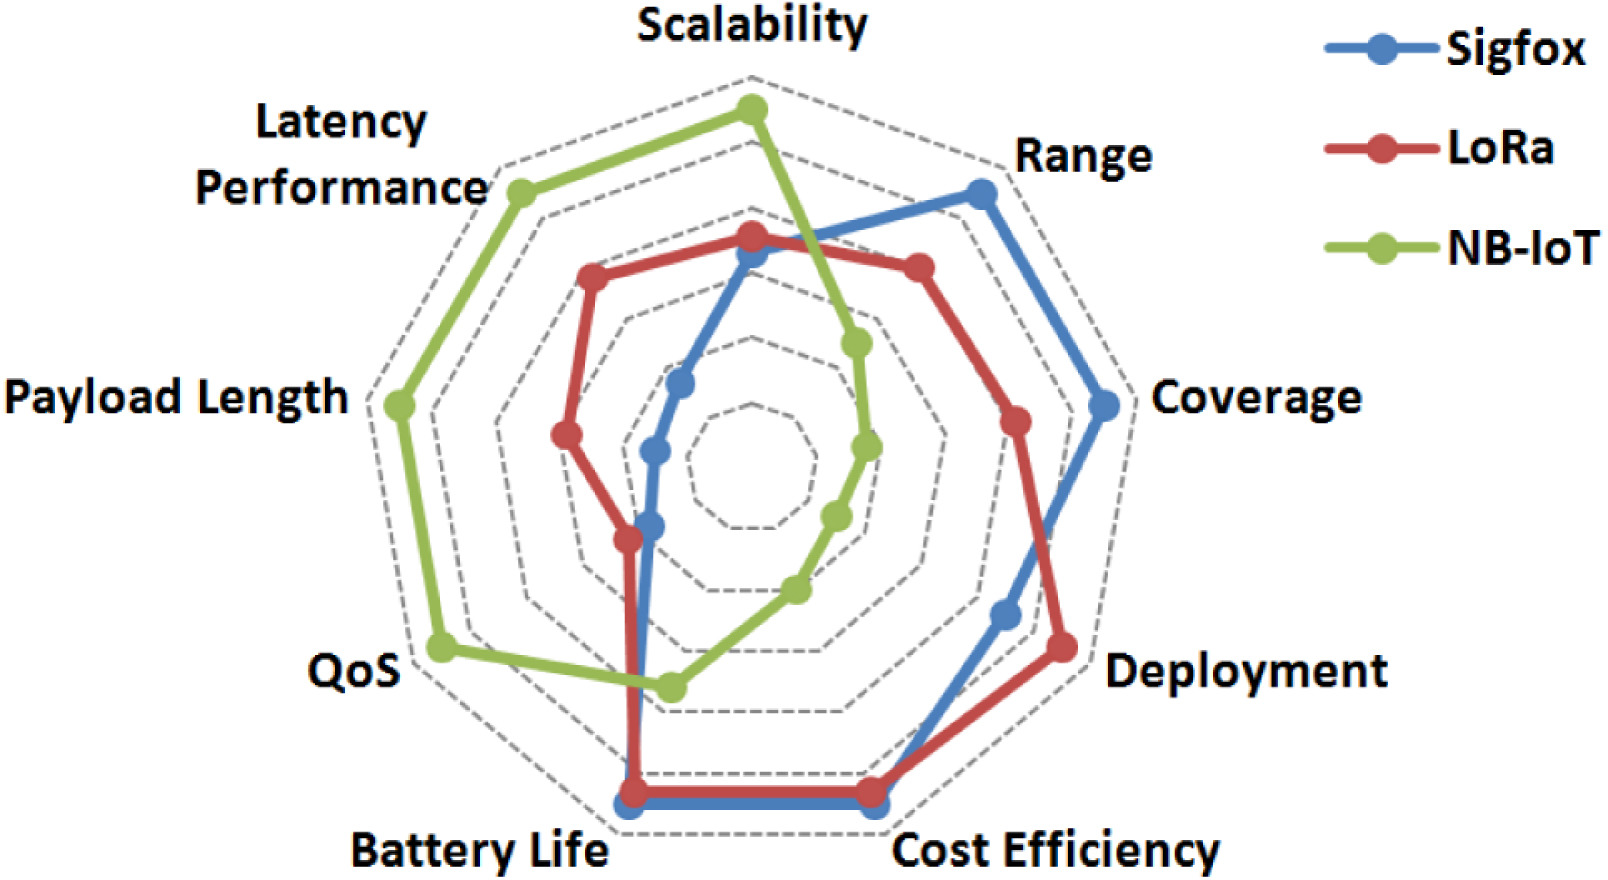
\includegraphics[width=.9\columnwidth]{LPWANcomparrison.jpg}}
  \caption{Respective advantages of Sigfox, LoRa, and NB-IoT in terms of IoT factors. \cite{mekki2019comparative}}
  \label{fig:LPWAN_comparison}
\end{figure}

\begin{figure}[htbp]
  \centering
  \fbox{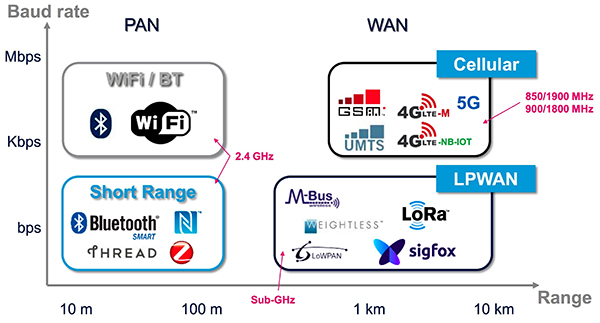
\includegraphics[width=.9\columnwidth]{NetworkRangeDataRateGraph.jpg}}
  \caption{Data rate vs range for different network technologies. \cite{evanczukspeed}}
  \label{fig:LPWAN_data_rate_range}
\end{figure}

\section{Conclusion}
\label{sec:Coclusion}


%%
%% The acknowledgments section is defined using the "acks" environment
%% (and NOT an unnumbered section). This ensures the proper
%% identification of the section in the article metadata, and the
%% consistent spelling of the heading.
\begin{acks}
  This is where you thank those who helped you better understand the material
  and gave you helpful feedback on the paper, usually including your adviser.
  This is not a place to thank your family, your significant other or your best friend,
  or anyone else  for moral support or yummy cookies.
\end{acks}

%%
%% The next two lines define the bibliography style to be used, and
%% the bibliography file.
\bibliographystyle{ACM-Reference-Format}
\bibliography{CBeaneSeniorSem}


\end{document}
\endinput
%%
%% End of file `sample-sigplan.tex'.
